% !TeX root = ../main.tex

\chapter{基于属性的访问控制系统}

\section{系统框架}

\begin{figure}
\centering
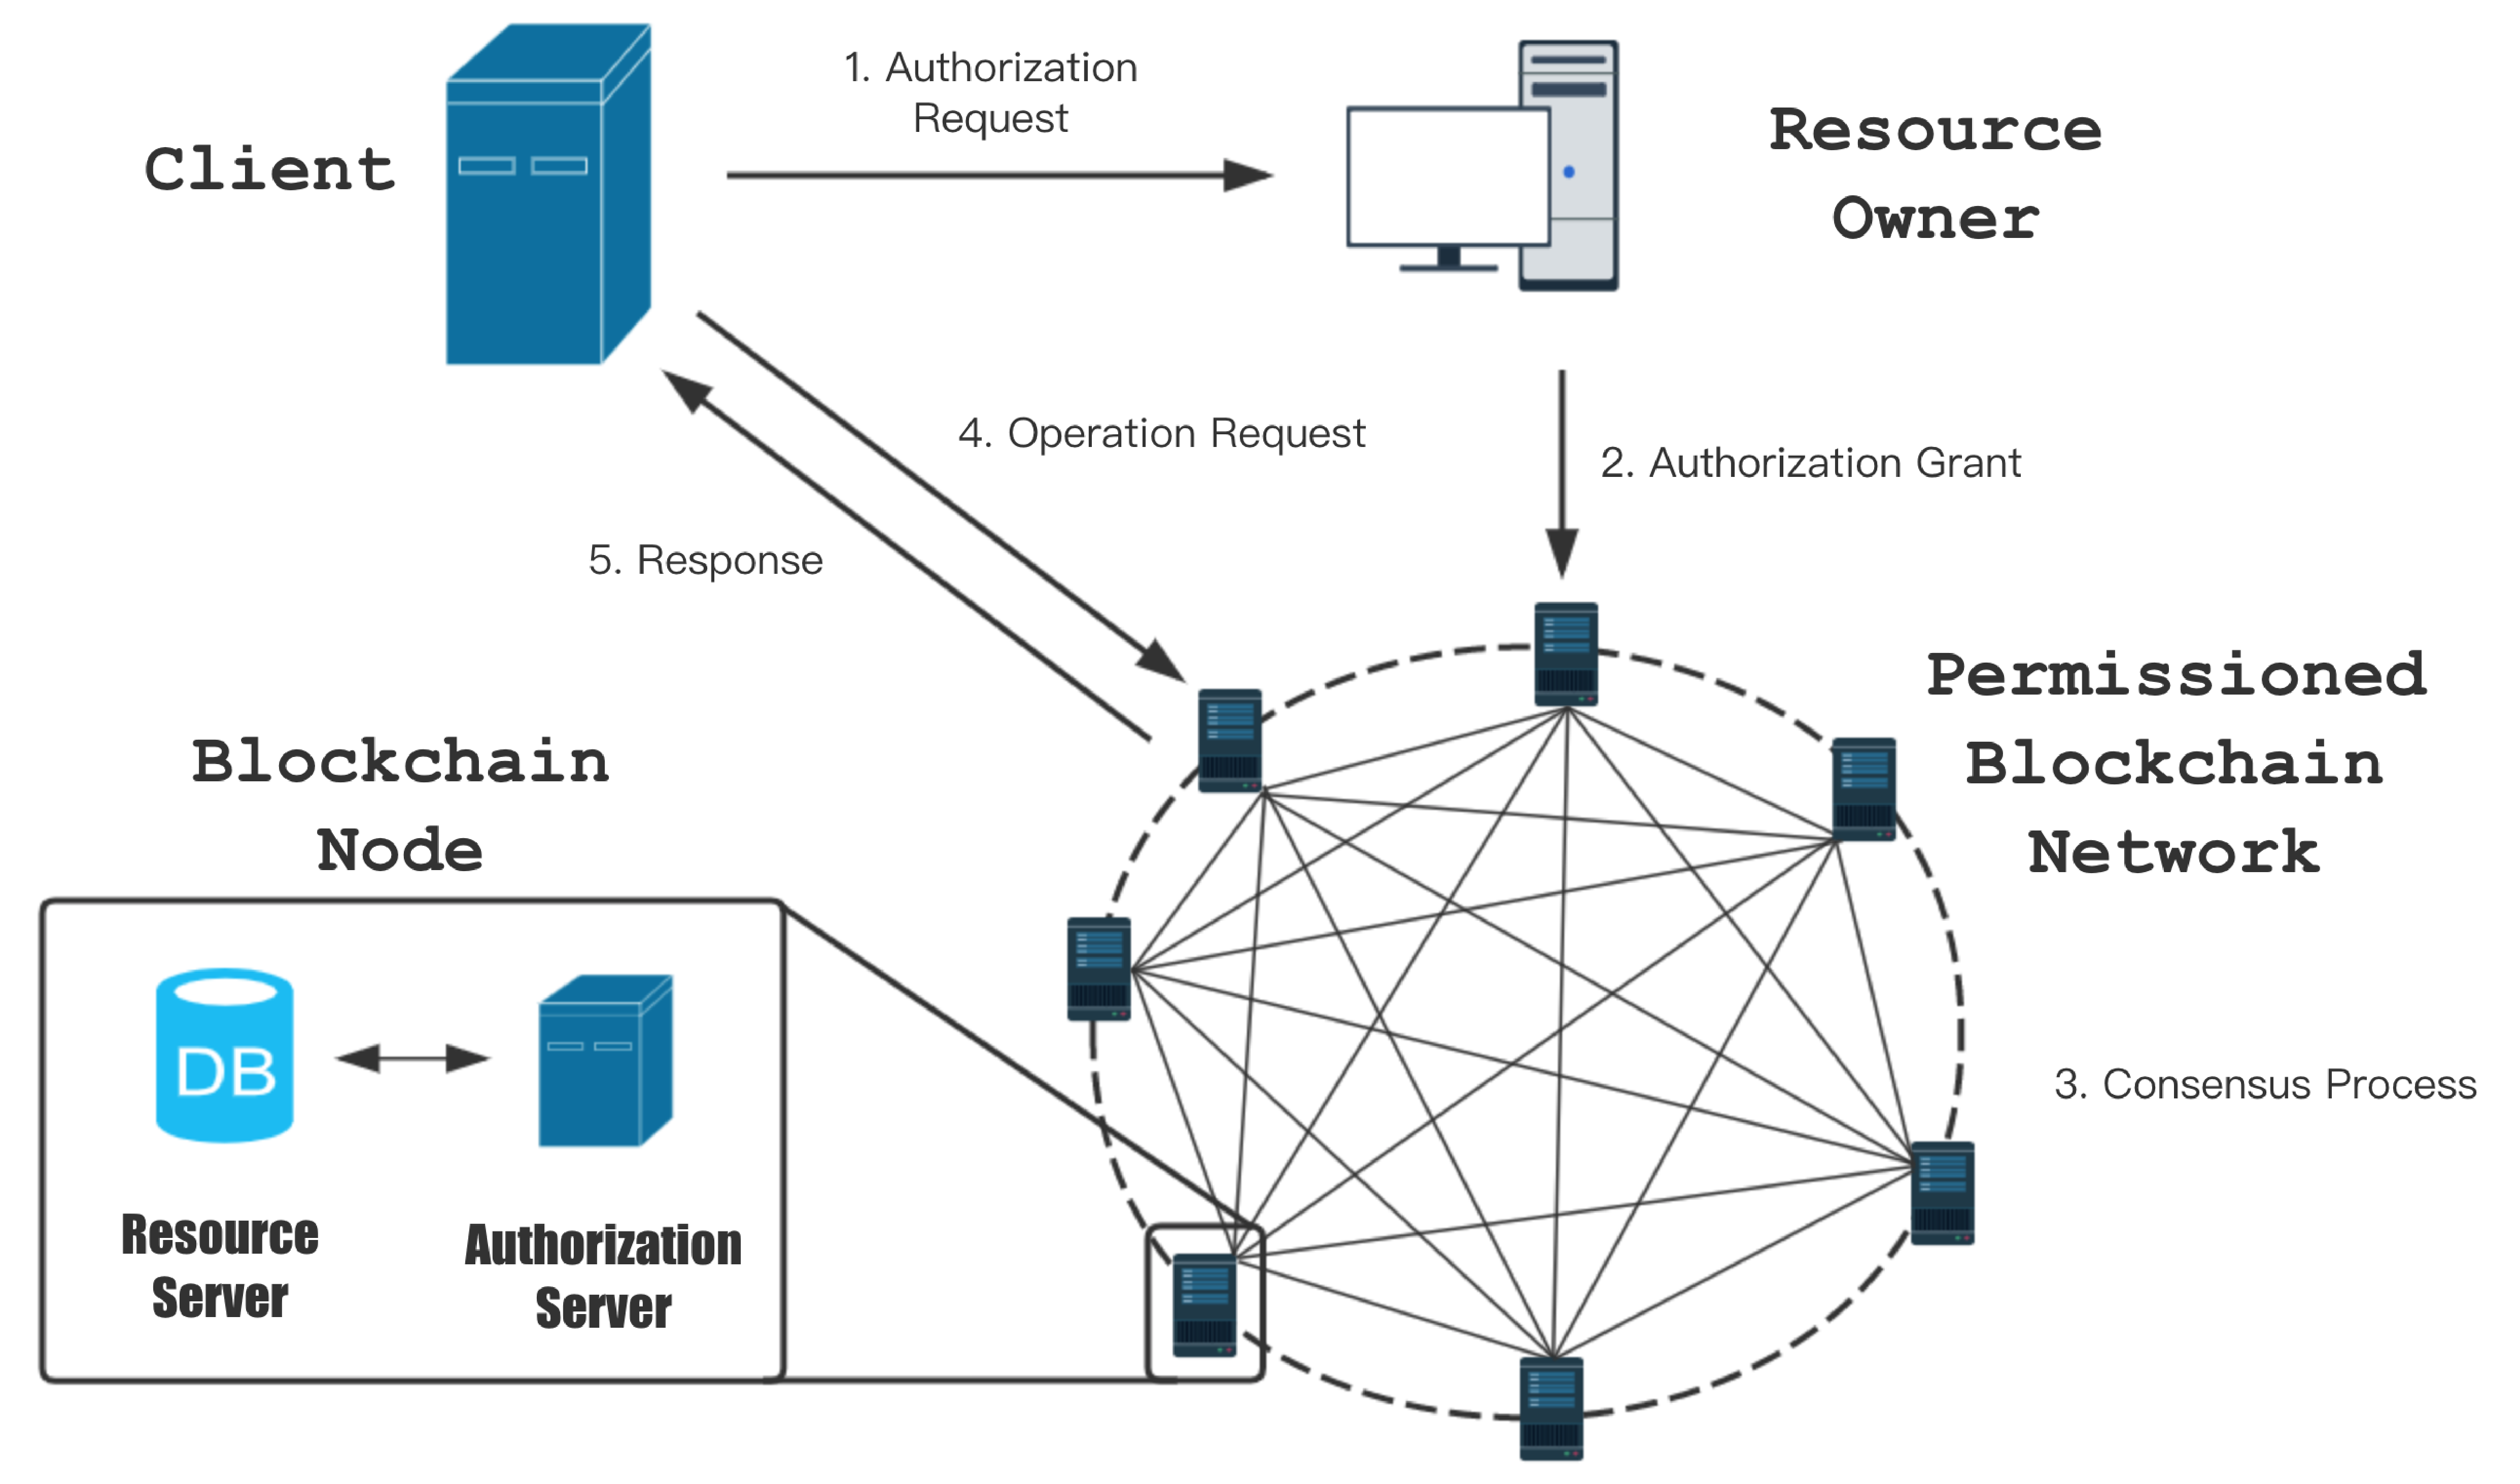
\includegraphics[width=11cm]{figures/archi.eps}
\caption{The Architecture of Decentralized Authorization and Authentication}
\label{fig:framework}
\end{figure}

通过运用区块链技术和基于属性的访问控制模型,我们提出了一个联盟链架构,类似OAuth框架用于第三方授权和认证。图\ref{fig:framework}给出了架构设计和工作流程的概述。该系统包含三类角色,“客户端”作为资源请求者,它请求资源所有者进行授权,并最终请求区块链节点访问资源。“资源所有者”在区块链节点上存储资源,在需要时授予“客户端”访问受保护资源的权限。该架构以联盟网络代替OAuth框架中的中心化认证服务器和资源服务器,该网络中的每个节点具有平等的地位,各自存储用户特定资源并且共同参与用户数据授权和身份验证数据的存储和管理。每个节点由资源服务器和授权服务器组成,其中资源服务器存储用户资源并使用基于属性的访问控制策略进行认证管理。当接收到操作请求时,资源服务器可以使用访问控制策略列表对请求中的各项属性进行身份验证。授权服务器与其他节点的授权服务器共同管理区块链,将用户发起的授权数据存储在区块链中,并且它可以根据区块链对资源服务器提供用于身份验证的各账户的主体属性。

\begin{description}
  \item[\textbf{资源所有者}] 资源所有者存储自己的资源在资源服务器,并在需要时授予客户端访问受保护资源的权限。
  \item[\textbf{客户端}] 客户端指资源请求者,通过向资源所有者发送请求获取授权,并访问资源服务器获取资源。不同于OAuth框架中客户端需要提前注册,任何用户都可以独自创建账户作为客户端。
  \item[\textbf{区块链节点}] 联盟链网络由若干互联的区块链节点组成。每个节点包含授权服务器和资源服务器。其中资源服务器保管资源所有者存储的部分资源,并采用基于属性的访问控制模型验证操作请求。所有节点的授权服务器共同运行共识协议,管理记录资源所有者对客户端的授权,并维护账户的属性状态。
\end{description}

该系统在以下几个方面提高了OAuth等中心化访问控制架构的安全性:

\begin{enumerate}
  \item OAuth框架中,第三方平台需要事先在授权服务器进行注册获取客户端密码,然后将客户端密码发送到授权服务器验证身份并获取访问令牌。一旦攻击者入侵了中心化的授权服务器,就可以通过发布伪造的令牌,从而伪装成任何用户访问资源服务器中受保护的资源。该系统中采用的非对称加密系统和去中心化架构可以有效降低攻击的严重程度。在共识达成一致的联盟网络中,攻击者只能访问被入侵的服务器中存储的资源。由于用于电子签名的私钥由用户本地生成并保管,用户发起的操作和授权不能被伪造,从而保护了存储在其他平台上的资源。

  \item 系统中使用的数字签名可以防止跨站请求伪造(Cross-Site Request Forgery,CSRF)攻击。OAuth框架在多个平台广泛实现,并使用重定向URL连接不同的平台,这可能会带来CSRF攻击。例如,它通常用于中心化平台和第三方平台之间的帐户绑定。攻击者可以先访问授权服务器,获得绑定第三方平台和中心化平台账户的访问令牌,然后诱使用户向第三方平台发送绑定请求,并提前提供攻击者获得的令牌。因此,攻击者可以通过中心化平台的账号访问第三方平台上的用户资源。在我们的系统中,用户发送的所有授权和操作都需要进行数字签名,这样才能保证授权的来源。
\end{enumerate}

\section{协议流程}
\label{sec:protocols}
本节介绍此框架中的协议。整个协议主要分为5个步骤,分别对应于图\ref{fig:framework}中的工作流程。每一步的详细信息在\ref{sec:protocols}中描述,具体步骤如下:

\begin{enumerate}
  \item 客户端向资源所有者发送$Authorization Request$,其中主要包含客户端的地址和请求授权的属性。
  \item 资源所有者检查$Authorization Request$,如果同意则生成相应的$Authorization Grant$并且发送给任何区块链节点。
  \item 如果接收到的$Authorization Grant$有效,则区块链节点将接受并在网络中传播它。共识过程结束后,授权将被打包到一个新的区块中,并记录到区块链上。
  \item 获得授权后,客户端找到存储需要访问资源的区块链节点,并发送$Operation Request$给该节点的资源服务器。
  \item 资源服务器根据授权服务器提供区块链上账户的主体属性,存储的资源属性以及基于属性的访问控制策略来验证$Operation Request$,根据验证结果回应客户端。
\end{enumerate}

接下来将详细介绍各步骤的细节。首先介绍后续涉及的一些密码学表示,对于消息$m$,我们定义$H(m)$表示$m$的哈希值,并且用$\langle m \rangle_{\sigma_{i}}$ 表示消息 $m$ 以及节点$i$对 $H(m)$ 的签名。可以用于验证该消息的真实来源以及是否在传输中被篡改。

\subsection{区块链和属性状态}

该系统中,区块链是用来存储授权记录的基本数据结构,每个区块记录一系列授权信息,每个授权信息包括发送方地址,接收方地址,授权属性,授权有效期以及用于验证的签名等信息。为了在本系统中,我们采用了以太坊项目中的账户状态机制,而非比特币项目中的未花费输出(Unspent Transaction Output, UTXO)机制,因为状态设计更适合ABAC模型。我们将账户中的余额等信息修改为属性状态,区块链记录每个账户拥有的所有属性以及nonce值,每个属性包括属性名和有效期。全局状态指所有帐户的信息。根据区块链,我们可以计算包含地址、nonce和属于地址的属性状态的每个帐户的状态。状态保存在内存中,可用于验证授权或操作。在区块链上添加新块时,全局状态将根据新块中的授权进行更改。我们可以将全局状态视为区块链的当前结果。对于帐户状态中的nonce值,每个帐户都有一个nonce值,其值为0。地址D的一次授权记录在区块链上时,地址D的一次授权将增加1。任何与nonce值不匹配的授权都将被拒绝。这可以防止重播攻击,因为一旦在区块链上记录了授权,就不能再接受它,因为增加了nonce值。

\subsubsection{对授权的验证}

联盟链网络中的节点收到客户端发送的授权后,首先验证该授权,如果通过则添加到授权池中,等待打包进新区块。更多细节在算法 \ref{alg:authVerify}中介绍。

 \begin{algorithm}
 \floatname{algorithm}{Algorithm}
 \caption{授权验证}\label{alg:authVerify}
   \begin{algorithmic}[!htbp]
   \renewcommand{\algorithmicrequire}{\textbf{Input:}}
   \renewcommand{\algorithmicensure}{\textbf{Output:}}
   \REQUIRE $Authorization$
   \ENSURE  $Verification$
    \STATE $Sender$, $Receiptor$, $Attributes$, $nonce$, $Signature \gets Parse(Authorization)$
    \STATE $AuthorizationHash \gets Hash(Authorizaton)$
    \IF {$CheckSignature(Sender, Hash, Signature) \ne true$}
      \RETURN $false$
    \ENDIF
    \STATE $SenderState \gets GetStateFromAddress(Sender)$
    \IF {$nonce < SenderState.nonce$}
      \RETURN $false$
    \ENDIF
    \FOR {$each Attribute \in Attributes$}
      \IF {$SenderState.VerifyAttribute(Attribute) \ne true$}
        \RETURN $false$
      \ENDIF
    \ENDFOR
    \STATE AddAuthorizationToPool(Authorization)
   \RETURN $true$
   \end{algorithmic}
 \end{algorithm}

\subsubsection{对操作请求的验证}

资源服务器能获取同一节点中授权服务器同步的区块链状态,因此,当收到客户端对资源的操作请求时,资源服务器首先通过授权服务器获取客户端地址拥有的属性,即主体属性,然后获取被访问资源对应的客体属性,操作请求对应的操作属性,以及当前的环境属性(即时间戳)。最后根据自己存储的属性访问控制列表对所有属性进行计算得到是否允许该操作。具体过程如算法 \ref{alg:opVerify}所示.

 \begin{algorithm}
 \floatname{algorithm}{Algorithm}
 \caption{验证操作}
   \begin{algorithmic}[H]\label{alg:opVerify}
   \renewcommand{\algorithmicrequire}{\textbf{Input:}}
   \renewcommand{\algorithmicensure}{\textbf{Output:}}
   \REQUIRE $Operation$
   \ENSURE  $Verification$
    \STATE $Sender$, $OpCode$, $Obj$, $nonce$, $Timestamp$, $Signature \gets Parse(Operation)$
    \STATE $OperationHash \gets Hash(Operation)$
    \IF {$CheckSignature(Sender, Hash, Signature) \ne true$}
      \RETURN $false$
    \ENDIF
    \STATE $SenderState \gets GetStateFromAddress(Sender)$
    \IF {$nonce < SenderState.nonce$}
      \RETURN $false$
    \ENDIF
    \STATE$SubAttributes \gets GetAttrFromAddress(Sender)$
    \STATE$ObjAttributes \gets GetAttrFromObject(Obj)$
    \STATE$OpAttributes \gets GetAttrFromOpCode(OpCode)$
    \STATE$EnvAttributes \gets Timestamp$
    \FOR {$each Policy \in Policies do$}
      \IF {$Policy.Match$($SubAttributes$, $ObjAttributes$, $OpAttributes$, $EnvAttributes$) = $true$}
        \RETURN $true$
      \ENDIF
    \ENDFOR
   \RETURN $false$
   \end{algorithmic}
 \end{algorithm}

\subsubsection{区块生成算法}

联盟网络中的节点会将一段时间内接受到的授权信息打包到一个新区块中,在比特币系统中这个时间间隔是10分钟,而在以太坊中是15秒,动态调整的具体方法在前文章节\ref{subsec:work-proof}中有所介绍。而在本系统中,为了保障访问控制系统的延迟可接受,我们设置区块间隔为2秒,区块生成的具体算法在算法\ref{alg:blockGeneration}中介绍。

 \begin{algorithm}
 \floatname{algorithm}{Algorithm}{}
 \caption{Block Generation}\label{alg:blockGeneration}
   \begin{algorithmic}[!htbp]
   \renewcommand{\algorithmicrequire}{\textbf{Input:}}
   \renewcommand{\algorithmicensure}{\textbf{Output:}}
   \REQUIRE $AuthorizationPool, AUTH\_LIMIT, PreviousBlock$
   \ENSURE  $Verification$
    \STATE $auths \gets ChooseAuths(AuthorizationPool, AUTH\_LIMIT)$
    \STATE $prevHash \gets H(PreviousBlock)$
    \STATE $timestamps \gets CurrentTime()$
    \STATE $newBlock \gets NewBlock(prevHash, auths, timestamps)$
   \RETURN $newBlock$
   \end{algorithmic}
 \end{algorithm}

\subsection{改进的PBFT共识算法}

在前文第\ref{subsec:traditional-consensus}节中,我们介绍了多种一致性算法,用于保证分布式节点间数据的一致性,其中拜占庭容错算法能提供拜占庭式容错(BFT)。实用的拜占庭容错算法(PBFT)于1999年提出,减少了BFT的时间和通信复杂度,并已应用于区块链领域的超级账本项目中。我们在访问控制系统中采用了改进的PBFT算法。区块链网络广播中的节点向其他节点发送请求。经过一段时间后,主节点将合法请求打包成块。然后将该块广播到网络中,与其他节点取得一致的结果。

\subsubsection{节点和视图}

主节点、备份节点和视图更改基本采用PBFT算法的设计。但存在如下差异,PBFT算法中的主节点在接收到来自客户端的请求时开始协商过程。在这个系统中,主节点每2秒启动一次协商,并将最多1000个授权打包到一个新区块中。当备份节点发现主节点似乎发生故障或被攻击时,将发生视图更改,这与PBFT算法中的视图变化相同。除此之外,当一段时间后,系统中的节点也会自动进行视图更改。这可以防止来自恶意主节点的黑名单攻击。在区块链系统中,生成新块的节点可以选择其中包含的事务以及先后顺序,恶意节点可以拒绝打包黑名单中帐户的事务。因此,不断的视图更改可以防止来自恶意主节点的黑名单攻击。

\subsubsection{预准备阶段}

当一个新区块过程开始,所有节点进入预准备阶段。这一阶段中,主节点从授权池中选择一系列合法的授权,并且打包到一个新区块中。然后,主节点广播预准备信息$\langle PRE$-$PREPARE, v, i, block \rangle_{\sigma_{i}}$ 给所有备份节点,其中 $v$ 表示当前的视图编号,$i$ 表示主节点的节点编号。具体预准备信息$pre$-$prepare$的创建如算法\ref{alg:preprepareGen}所示。

 \begin{algorithm}
 \floatname{algorithm}{Algorithm}
 \caption{生成预准备信息}\label{alg:preprepareGen}
   \begin{algorithmic}[H]
   \renewcommand{\algorithmicrequire}{\textbf{Input:}}
   \renewcommand{\algorithmicensure}{\textbf{Output:}}
   \REQUIRE $blockchain, authorizationPool, AUTH\_LIMIT,$ $sk, viewID$
   \ENSURE  $pre$-$prepare$
    \STATE $prevBlock \gets blockchain.LastBlock()$
    \STATE $block$ $\gets$ $BlockGenration(prevBlock, AUTH\_LIMIT,$ $authorizationPool)$
    \STATE $pre$-$prepare \gets NewRequest(viewID, block)$
    \STATE $signature \gets sk.Sign(request)$
    \STATE $pre$-$prepare.Signature \gets signature$
   \RETURN $pre$-$prepare$
   \end{algorithmic}
 \end{algorithm}


当备份节点接受到主节点发送的预准备信息$pre$-$prepare$后,验证过程如算法\ref{alg:prepreVerify}所示。如果通过验证,备份节点将接受该信息并进入准备阶段。否则,该节点可以认为主节点被恶意控制或者宕机,将会发起视图切换,请求选举出下一个正常节点作为新的主节点。

 \begin{algorithm}
 \floatname{algorithm}{Algorithm}
 \caption{验证预准备信息}
   \begin{algorithmic}[H]\label{alg:prepreVerify}
   \renewcommand{\algorithmicrequire}{\textbf{Input:}}
   \renewcommand{\algorithmicensure}{\textbf{Output:}}
   \REQUIRE $pre$-$prepare$, $N$, $ViewID$, $i$, $PkList$
   \ENSURE  $Verification$
    \STATE $viewID$, $nodeID$, $timestamps$, $signature \gets Parse(pre$-$prepare)$
    \IF {$viewID \ne ViewID$}
      \RETURN $false$
    \ENDIF

    \IF {$nodeID \ne ViewID \% N$}
      \RETURN $false$
    \ENDIF

    \STATE $hash \gets H(pre$-$prepare)$
    \IF {$CheckSignature(PkList[i], hash, signature) \ne true$}
      \RETURN $false$
    \ENDIF
   \RETURN $true$
   \end{algorithmic}
 \end{algorithm}

\subsubsection{准备阶段}

如果备份节点 $i$ 接受了预准备信息$pre$-$prepare$,该节点进入准备阶段。节点$i$生成准备信息$\langle PRE$-$PARE, v, i, blockHash\rangle_{\sigma_{i}}$,其中视图编号$v$和预准备信息中的视图编号一致,$i$ 表示该备份节点的节点编号,$blockHash$ 表示预准备信息$pre$-$prepare$中包含区块的哈希值。具体细节在算法\ref{alg:prepareGen}中介绍。然后该备份节点将生成的准备信息 $prepare$广播给其他所有节点,包括主节点在内。一旦某个节点从不同的来源节点(包括自己)接收到$2f+1$个拥有相同$v$和 $blockHash$的准备信息,该节点将会进入承诺阶段。

 \begin{algorithm}
 \floatname{algorithm}{Algorithm}
 \caption{生成准备信息}
   \begin{algorithmic}[H]\label{alg:prepareGen}
   \renewcommand{\algorithmicrequire}{\textbf{Input:}}
   \renewcommand{\algorithmicensure}{\textbf{Output:}}
   \REQUIRE $pre$-$prepare, nodeID, sk, NeighborList$
   \ENSURE  $prepare$

    \STATE $blockHash$ $\gets$ $H(pre$-$prepare.Block)$

    \STATE $viewID \gets pre$-$prepare.ViewID$
    \STATE $prepare \gets NewPrepare(viewID, nodeID, blockHash)$
    \STATE $signature \gets sk.Sign(prepare)$
    \STATE $prepare.Signature \gets signature$
   \RETURN $prepare$
   \end{algorithmic}
 \end{algorithm}

\subsubsection{承诺阶段}

进入承诺阶段的节点获知网络中大部分正常节点(至少f+1个)已经接受该信息。节点$i$将生成并广播承诺信息$\langle COMMIT, v, i, blockHash \rangle_{\sigma_{i}}$ 给所有节点,表明该节点将接受这一新区块作为共识结果。承诺的生成过程如算法\ref{alg:commitGen}所示。

 \begin{algorithm}
 \floatname{algorithm}{Algorithm}
 \caption{Commit Generation}
   \begin{algorithmic}[H]\label{alg:commitGen}
   \renewcommand{\algorithmicrequire}{\textbf{Input:}}
   \renewcommand{\algorithmicensure}{\textbf{Output:}}
   \REQUIRE $prepare, nodeID, blockHash, sk$
   \ENSURE  $commit$

    \STATE $viewID \gets prepare.ViewID$
    \STATE $blockHash \gets prepare.blockHash$
    \STATE $commit \gets NewCommit(viewID, nodeID, blockHash)$
    \STATE $signature \gets sk.Sign(prepare)$
    \STATE $commit.Signature \gets signature$
   \RETURN $commit$
   \end{algorithmic}
 \end{algorithm}

当某个节点从不同来源节点接收到 $2f+1$个合法的承诺信息,该节点可以确认该新区块至少被$f+1$个正常节点接受,因为在接收的$2f+1$个承诺信息中,至多只有$f$个来源于拜占庭节点。然后该节点可以将该区块记录在区块链上,并更新账户状态。

\section{原型实现}

\begin{figure}
\centering
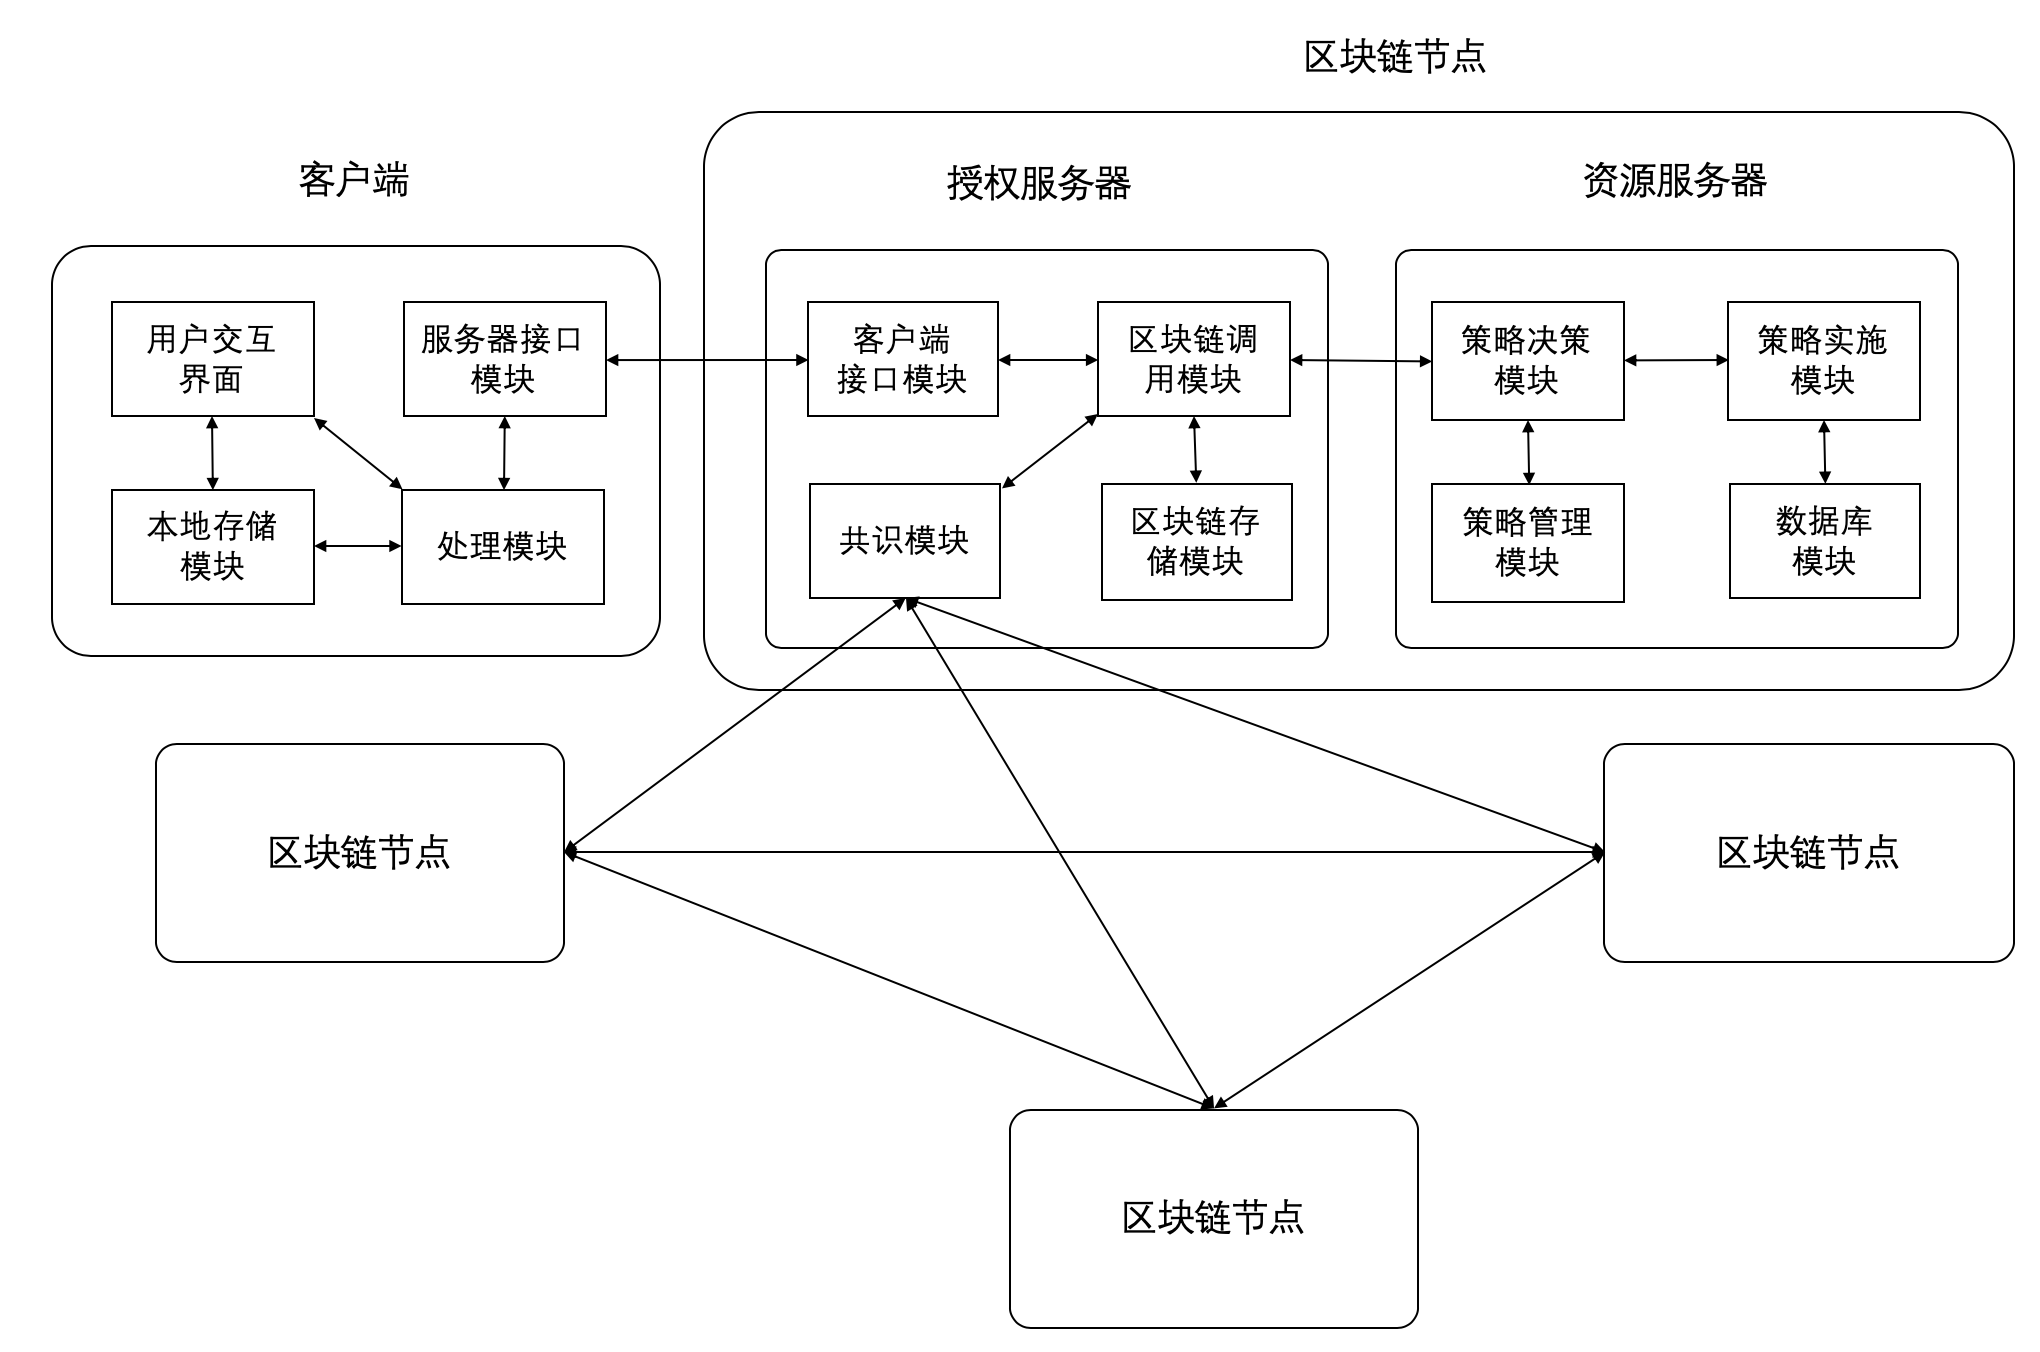
\includegraphics[width=12cm, keepaspectratio]{figures/implementation.png}
\caption{The Implementation of Prototype}
\label{fig:implementation}
\end{figure}

如图\ref{fig:implementation}所示,基于上述协议,我们实现了一个原型系统用于验证设计框架和协议的可行性,并且评估性能和延迟等重要指标。

这一系统采用Go程序语言实现,因为Go语言的并发机制(goroutines和channel通信)帮助构建高性能的网络应用,能提升访问控制系统的性能。为了简化实现,资源服务器采用键值对数据库leveldb存储资源,实际上可以采用现有的任意数据库实现。在区块链网络中,节点间的通信采用HTTP协议实现,未来还可以考虑采用UDP协议提升性能。

\begin{itemize}
  \item 客户端:与框架中客户端角色不同,这里实现的客户端用于用户管理自己的账户和密钥,授权其他用户,以及操作可访问的资源。该客户端可以生成并签名授权请求和操作请求,并且和服务器节点进行交互。
  \item 授权服务器: 授权服务器主要实现以下四个模块功能:
    \begin{enumerate}
      \item 与客户端交互模块:该模块接受客户端的授权请求和操作请求并转发给处理器模块。
      \item 区块链模块:该模块与其他服务器进行通信,发送并接受区块链相关信息,包括授权请求,区块数据等。同时负责区块数据以及状态数据的存储和更新。
      \item 共识模块:该模块发送并接受改进的PBFT协议中的相关消息,包括预准备信息,准备信息,承诺信息,更新视图等。采用多个定时器通过管道实现,保障在限定时间内达成共识产生新区块。
      \item 处理器模块:该模块处理从客户端或者其他节点接收到的消息,运行前文介绍的区块生成和验证算法。
    \end{enumerate}
  \item 资源服务器:资源服务器主要由以下两个模块组成:
    \begin{enumerate}
      \item 区块链模块:该部分验证授权服务器同步的区块链信息,并且管理所有账户的状态数据。
      \item 访问控制模块:该模块保存基于属性的访问控制列表,并在接收到操作请求时对请求进行验证。
      \item 数据库模块:该模块管理用户存储资源的数据库,并根据访问控制模块的验证结果对数据进行操作。
    \end{enumerate}
\end{itemize}

\begin{figure}
\centering
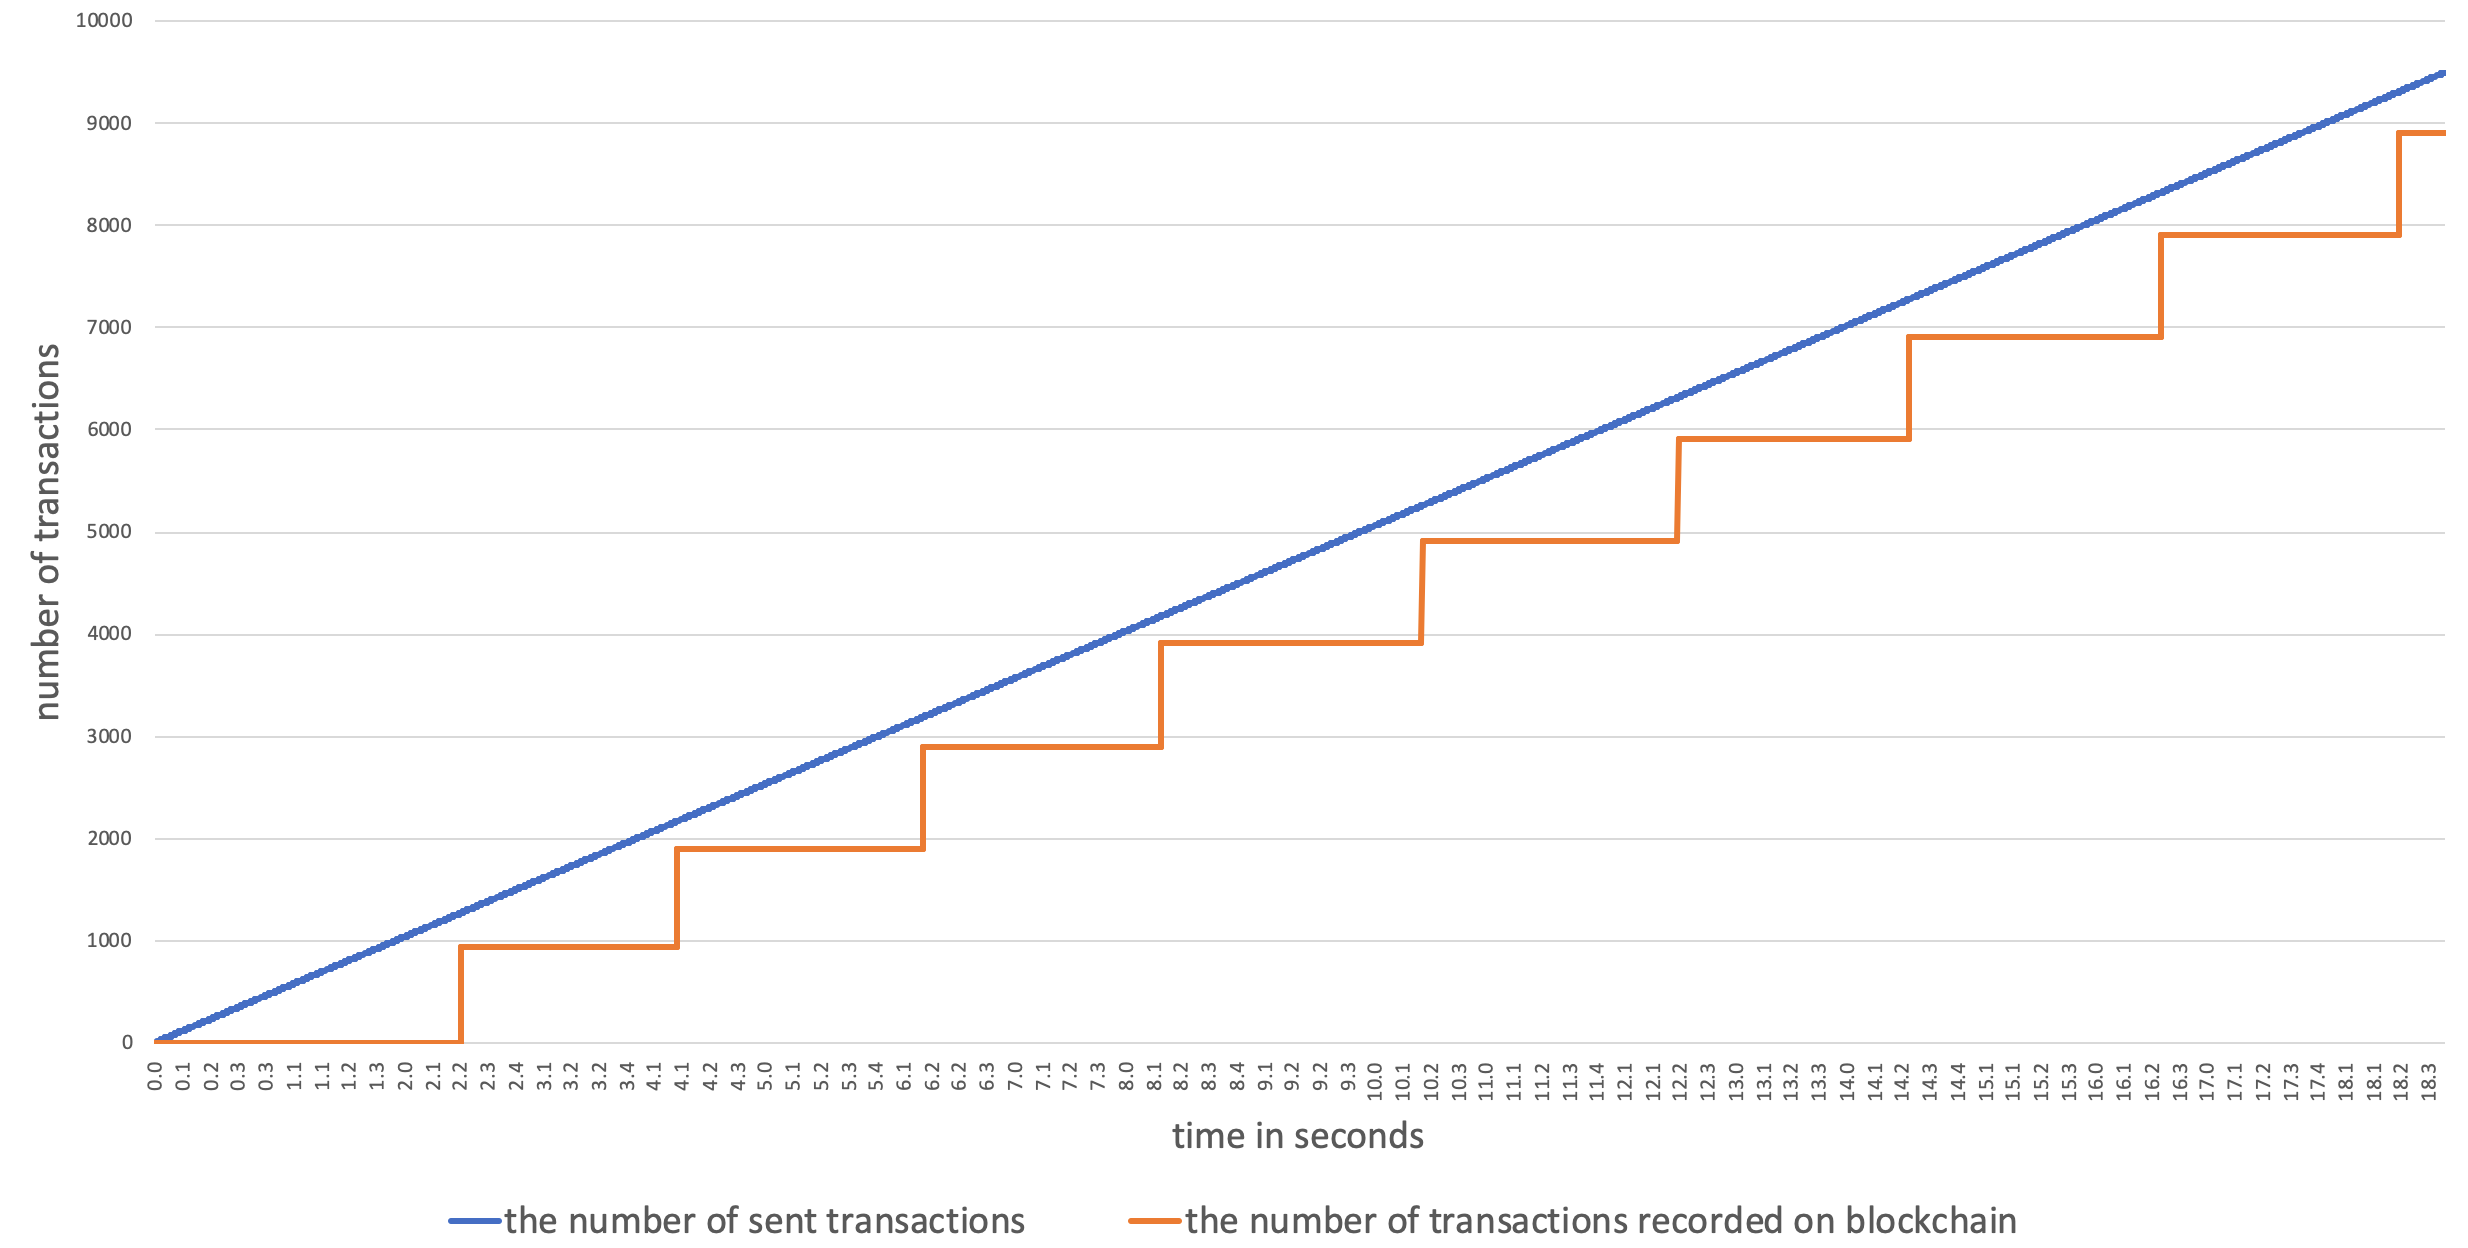
\includegraphics[width=12cm, keepaspectratio]{figures/performance.png}
\caption{Performance Testing}
\label{fig:performance}
\end{figure}

我们在微软云平台上部署了四个区块链节点,每个节点采用标准的D2s v3型号服务器,拥有2 vCPU,2G内存以及1,000 MBps网络带宽。为了测试系统性能,我们生成了1000对公私钥对来模拟1000个用户,每个用户拥有不同的属性,还在随机用户之间生成了10000个随机的授权操作,用于模拟现实中的授权行为。

测试授权数据以每秒500个授权的速率发送给4个节点,区块链网络在大概21秒的时间里成功处理了这些请求。发送的分布时间如图\ref{fig:performance}所示。该网络每2秒生成一个新区块,并且每个区块最多包含1000个授权请求(这一限制设置在代码中)。每个区块包含的授权信息数量如图\ref{fig:performance}所示。实验证明了该系统可以达到每秒处理500个授权请求并且平均延迟在1秒左右,这说明该框架和协议可以应用于现实场景中。